\subsection{IFIT Subcellular Localisation During Interferon Induction and RSV Infection} \label{subsec:IFIT Subcellular Localisation During Interferon Induction and RSV Infection}
introduction for why we wanted to look at colocalisation of ifit durng infection and elsevere

To investigate this, we seeded A549, MDBK, and later BEAS2B cell lines on a 13 mm diameter glass coverslip in a 24-well plate in a initial concentration on 100,000 cells per well as described in Section \ref{sec:Cell Culture}. 24 hours post seeding these cells were either mock infected; treated with either human or bovine interferon alpha at concentrations of 1,000 international units per mL for the former or 5 ng/mL (these concentrations correspond to each other); or infected with either human or bovine wild-type RSV at MOI of 1. After 24 hours the samples were fixed with paraformaldehyde and prepared as described in Section \ref{sec:Confocal Microscopy} for the subsequent confocal microscopy analysis. The samples were stained with DAPI that allowed nuclear detection (consistently shown in yellow) and antibodies against RSV N protein (consistently shown in cyan) and the IFIT proteins (consistently shown in magenta). We used one specific antibody against each of IFIT1, IFIT3, and IFIT5, while we used two antibodies that we had access to against IFIT2. For the sake of simplicity, we will refer to these antibodies as IFIT2A and IFIT2B antibodies.

Figure \ref{fig:The Changes in Subcellular Localisation of Human IFITs in A549 Cells Subjected to hIFNa or hRSV} shows the subcellular localisation of human IFIT proteins in mock-, hIFN\(\alpha\)-, or human RSV-treated samples observed in A549 cell line. Human IFIT1 is cytoplasmic and nuclearly excluded in a basal state. Interestingly, hIFN\(\alpha\) stimulation does not alter this localisation pattern, neither the abundance of IFIT1 as detected by the intensity of the signal. During infection, IFIT1 stays cytoplasmic and excluded from nucleus with a possible colocalisation with N, on the outside of the IB structure. The intensity of staining is increased, especially in uninfected cells, suggesting hypothesis from Chapter \ref{ch:Assessment of Transcriptional Induction of Human IFITs in the Context of RSV} is correct. IFIT2A antibody shows hIFIT2 to be located in cytoplasmicly diffused but nuclearly excluded vesicular pattern, for both basal pattern and IFN\(\alpha\) induced pattern. The intensity between these two conditions appear to be equal. During hRSV infection, the overal intensity seems to decrease. The subcellular localisation also changes into a phenotype with less vesicules and inclusions inside the RSV IB structures. IFIT2B antibody on the other hand detects IFIT2 to be granular and cytoplasmic, while also showing to be excluded from the nucleus. Like with IFIT2A antibody, the intensity and localisation phenotype between mock and IFN\(\alpha\) treated cells is equal. During hRSV onfection, this antibody detect IFIT2 to be excluded from both the nucleus and the inclusion body, while retaining vesicular cytoplasmic stain. IFIT3 appears to be cytoplasmic with nuclear exclusion under basal conditions. After IFN\(\alpha\) treatment we can observe increase in the staining intensity and signs of IFIT3 nuclear translocation. During hRV infection IFIT3 seems to be evenly diffused throught the whole cell, including the RSV inclusion body and the nucleus. The intesity of staining during infection appears similar between IFN\(\alpha\) treated and hRSV infected cells. IFIT5 is also cytoplasmically located under basal conditions while being excluded rom the nucleus. During IFN\(\alpha\) treatment the phenotype and the intensity of the staining remain the same. Dyring hRSV infection, we can see uninfected cells displaying increased IFIT5 levels. With regards to the staining pattern, it remains cytoplasmic and excluded from both nucleus and RSV IB.

\begin{figure}
    \centering
    \includegraphics[width=1\linewidth]{08. Chapter 3/Figs/01. Localisation introduction/07. a549 merges.pdf}
    \caption[The Changes in Subcellular Localisation of Human IFITs in A549 Cells Subjected to hIFN\(\alpha\) or hRSV.]{\textbf{The Changes in Subcellular Localisation of Human IFITs in A549 Cells Subjected to hIFN\(\alpha\) or hRSV.} A549 cell were either mock treated, or treated with 1000 IU/mL of hIFN\(\alpha\) for 24 hours, or were infected with hRSV MOI 1 for 24 hours. Cells were fixed, and stained with DAPI (nuclei detection; yellow), anti-RSV N antibody (cyan), or with antibodies against IFIT proteins (magenta). Two antibodies against IFIT2 were used, termed IFIT2A and IFIT2B. Insets with magnified selections were created from infected images to more easily convey the underlying subcellular localisations.}
    \label{fig:The Changes in Subcellular Localisation of Human IFITs in A549 Cells Subjected to hIFNa or hRSV}
\end{figure}


Figure \ref{fig:The Changes in Subcellular Localisation of Bovine IFITs in MDBK Cells Subjected to bIFNa or bRSV} shows the subcellular localisation of bovine IFIT proteins in mock-, bIFN\(\alpha\)-, or bovine RSV-treated samples observed in MDBK cell line. Under basal conditions, bIFIT1 is located cytoplasmicly with nuclear exclusion. In some cells we can see vesicules located throught the cells. Upon bIFN\(\alpha\) stimulation we can see that the subcellular localisation remains unchanged. What changes is the overall intensity of staining. Samples infected with bRSV show cytoplasmic staining with nuclear and IB exclusion, without any ovious vesicules. Surrounding non-infected cells display increased IFIT1 signal, while infected cells show staioning intensity lower than what we observed with interferon stimulated cells. IFIT2A antibody detects bIFIT2 to be predonimantly cytoplasmic with concentrations in a proximity to nucleus which resemble the endoplasmic reticulum. This signal is also excluded from the nucleus. In interferon treaded cells, the overal pattern apperas to be the same with the exception of decreased staining intensity and decreased size of nucleraly proximal condensations. During bRSV infection we see results identical to wat was observed in A549 cell line. The cytoplasmic signal is greatly reduced and instead IFIT2 either colocalises with RSV N on the baundry of the IB, or concentrates inside the inclusion bodies as a inclusion. IFIT2B on the other hand shows bIFIT2 to be cytoplamic with vesicules present spread through the cytoplasm and nucleus under basal conditions. Unfortunately we lack the cells treated with bIFN\(\alpha\) that were stained with IFIT2B antibody. During bRSV infection, this antibldy shows bIFIT2 to have the same localisation and intensity as what was observed in mock cells. It also shows IFIT2 to be excluded from the IB structure. bIFIT3 appears to be localised in vesicules with cytoplasmic and nuclear localisation in both mock and bIFN\(\alpha\) treated cells. The intensity signal appears to be slightly stronger in the interferon treated samples. During bRSV infection IFIT3 subcellular localisation changes drasticaly. It is barely detectable in cytoplasm and nucleus with the expeption of strong intra inclusion body inclusions. There also appears to be vesicles inside the inclusion that resembles the IBAGs. Last but not least, bIFIT5 shows cytoplasmic localisation with vesicles diffused through the cytoplasm, weak nuclear staining and inclusion within nuclei, most probaly colocalising with the nucleololi. In the samples treated with bIFN\(\alpha\), we cna see that although the pattern of subcellular localisation stays the same, the intensity is increased, especially in the nucleus. Finally, in the cells infected with the bRSV, we can observe nuclear exclusion with inclusion within the nucleoi; cytoplasmic staining with no obvious either colocalisation nor exclusion with RSV IBs. We can also see the cytoplasmic vesicles observed previously, although only in non-infected cells. The intensity of the staining resembles the one of mock treated cells.

\begin{figure}
    \centering
    \includegraphics[width=1\linewidth]{08. Chapter 3/Figs/01. Localisation introduction/09. mdbk-merges-test.pdf}
    \caption[The Changes in Subcellular Localisation of Bovine IFITs in MDBK Cells Subjected to bIFN\(\alpha\) or bRSV.]{\textbf{The Changes in Subcellular Localisation of Bovine IFITs in MDBK Cells Subjected to bIFN\(\alpha\) or bRSV.} MDBK cell were either mock treated, or treated with 5 ng/mL of bIFN\(\alpha\) for 24 hours, or were infected with bRSV MOI 1 for 24 hours. Cells were fixed, and stained with DAPI (nuclei detection; yellow), anti-RSV N antibody (cyan), or with antibodies against IFIT proteins (magenta). Two antibodies against IFIT2 were used, termed IFIT2A and IFIT2B. Insets with magnified selections were created from infected images to more easily convey the underlying subcellular localisations.}
    \label{fig:The Changes in Subcellular Localisation of Bovine IFITs in MDBK Cells Subjected to bIFNa or bRSV}
\end{figure}

Taking these results together, we can see quite the range of subcellular localisations and interactions with the RSV inclusion bodies. One thing that is consistent between cell lines and IFITs is that the IFN\(\alpha\) does rarely cause localisation changes of human and bovine IFITs, rather leads to an increase of detected concentration or no difference comapred to mock-treated samples. The exeption is human IFIT3, where hIFN\(\alpha\) caused increased nuclear localisation and bovine IFIT2, detected by IFIT2A antibody, which showed decreased overall IFIT2 signal and reduced the observed ER-like staining pattern. Human and bovine IFIT1 are both cytoplasmic and excluded from nucleus. They also both seem to be more expressed in uninfected cells during infection. Bovine IFIT1 differs in the presence of cytoplasmic vesicles and the differential interaction with the IBs, it is excluded whilr human IFIT1 seems to colocalise with IB boundry. IFIT2 antibodies show differential results, which are quite consistent in the interaction with the IBs between the cell lines. IFIT2A antibody shows human and bovine IFIT2 to be interacting with the RSV IBs, although the nature seems to differ. Human IFIT2 seems to be forming intra-IB inclusions, while bovine IFIT2 is colocalised with the IB boundry. IFIT2B consistently detected IFIT2 to be excluded from the inclusion bodies in both cell lines. We also observed discrepancies between the basal localisation, noth between the antibodies and between the cell lines. In human cells, while IFIT2A is shown to be vesicular and IFIT2B displayed more granular cytoplasmic stain, in bovine cells lines IFIT2A antibody showed cytoplasmic stain with IFIT2 concentrations on structures proximal to the nucleus, IFIT2B showed a vesicular stain without these structures. The differntial staining of the two antibodies could be trough acting on two distinct IFIT2 epitopes and needs to be investigated further. IFIT3 signal also differed between the human and bovine cells, both in terms of basal localisation and the interaction with the RSV IBs. While human IFIT3 is cytoplasmic and nuclearly excluded under basal conditions, we detected nuclear translocation after stimulation with either IFN\(\alpha\) or hRSV. On the other hand, bovine IFIT3 is vesicular with nuclear staining under basal conditions, although the nuclear staining disapeared in bRSV infected cells. With regards to the RSV IB interaction, human IFIT3 seem to be diffused evenly throught the cytoplasm, nucleus and the IB structures, bovine IFIT3 formed intra-IB inclusions with the signs of IBAGs. Last but not least, we also see small differences between human and bovine IFIT5 staining. Both are basaly cytoplasmic and their intensity increases after IFN\(\alpha\), although bovine IFIT5 was observed to also localise in cytoplasmic vesicles, nuclei and for intra-nucleolar inclusions. During infection, both human and bovine IFIT5 was cytoplasmic and nuclearly excluded, although bovine IFIT5 still retained the intra-nucleolar inclusion. With regards to the interaction with RSV IBs, human IFIT5 was clearly excluded while we were not able to clearly determine the bovine IFIT5 interaction phenotype with bovine RSV IBs. 

Seeing the potentially intersting results with IFIT colocalisation with RSV IBs, we expanded our analysis with hRSV infections in BEAS2B cell line and systematically analysed 1727 IB sizes and their underlying interaction phenotype with the different IFIT proteins. We categorised the phenotypes solely based on the IFIT staining, but in the area of the image where a presence of inclusion body was confirmed by viral protein staining (N, P, or M2/1 proteins). Figure \ref{fig:Inclusion Bodies Within RSV Infected Cells: Zoom Sequence} shows the representative region of interest and its underlying location within the cell and within cellular population. Based on our observations, we decided to categorise the phenotypes in a following manner: \textbf{Diffusion} phenotype would be assigned if the IFIT signal would be equally spread through the area if interest; \textbf{Exclusion} phenotype, which would be assigned by a obvious, partial or full, decrease in signal within the boundry of IB; \textbf{Edge exclusion} phenotype would be assigned if the IFIT signal would be equally spread through the area if interest with the exeption of IB boundry, from which it would be excluded; \textbf{Inclusion} phenotype would be assignes if there was obvious increase in the IFIT signal within the boundry of IB; and \textbf{Colocalisation} phenotype, which would be assigned if the IFIT signal would be equally spread through the area if interest with the exeption of increased signal in the IB boundry. These main phenotypes were also simetimes supplemented by either their interaction, or the presence of spots within the IB boundry. For the former, a very common occurance was colocalisation accompanied by exclusion. This was when there was an obvious increase on the IB boundry compared to the surrounding signal, while also a marked decrease of signal from within the region of interest was present. For the latter, these spots were termed IBAGs, as we speculate that these structures could be inclusion body associated granules. 

\begin{figure}
    \centering
    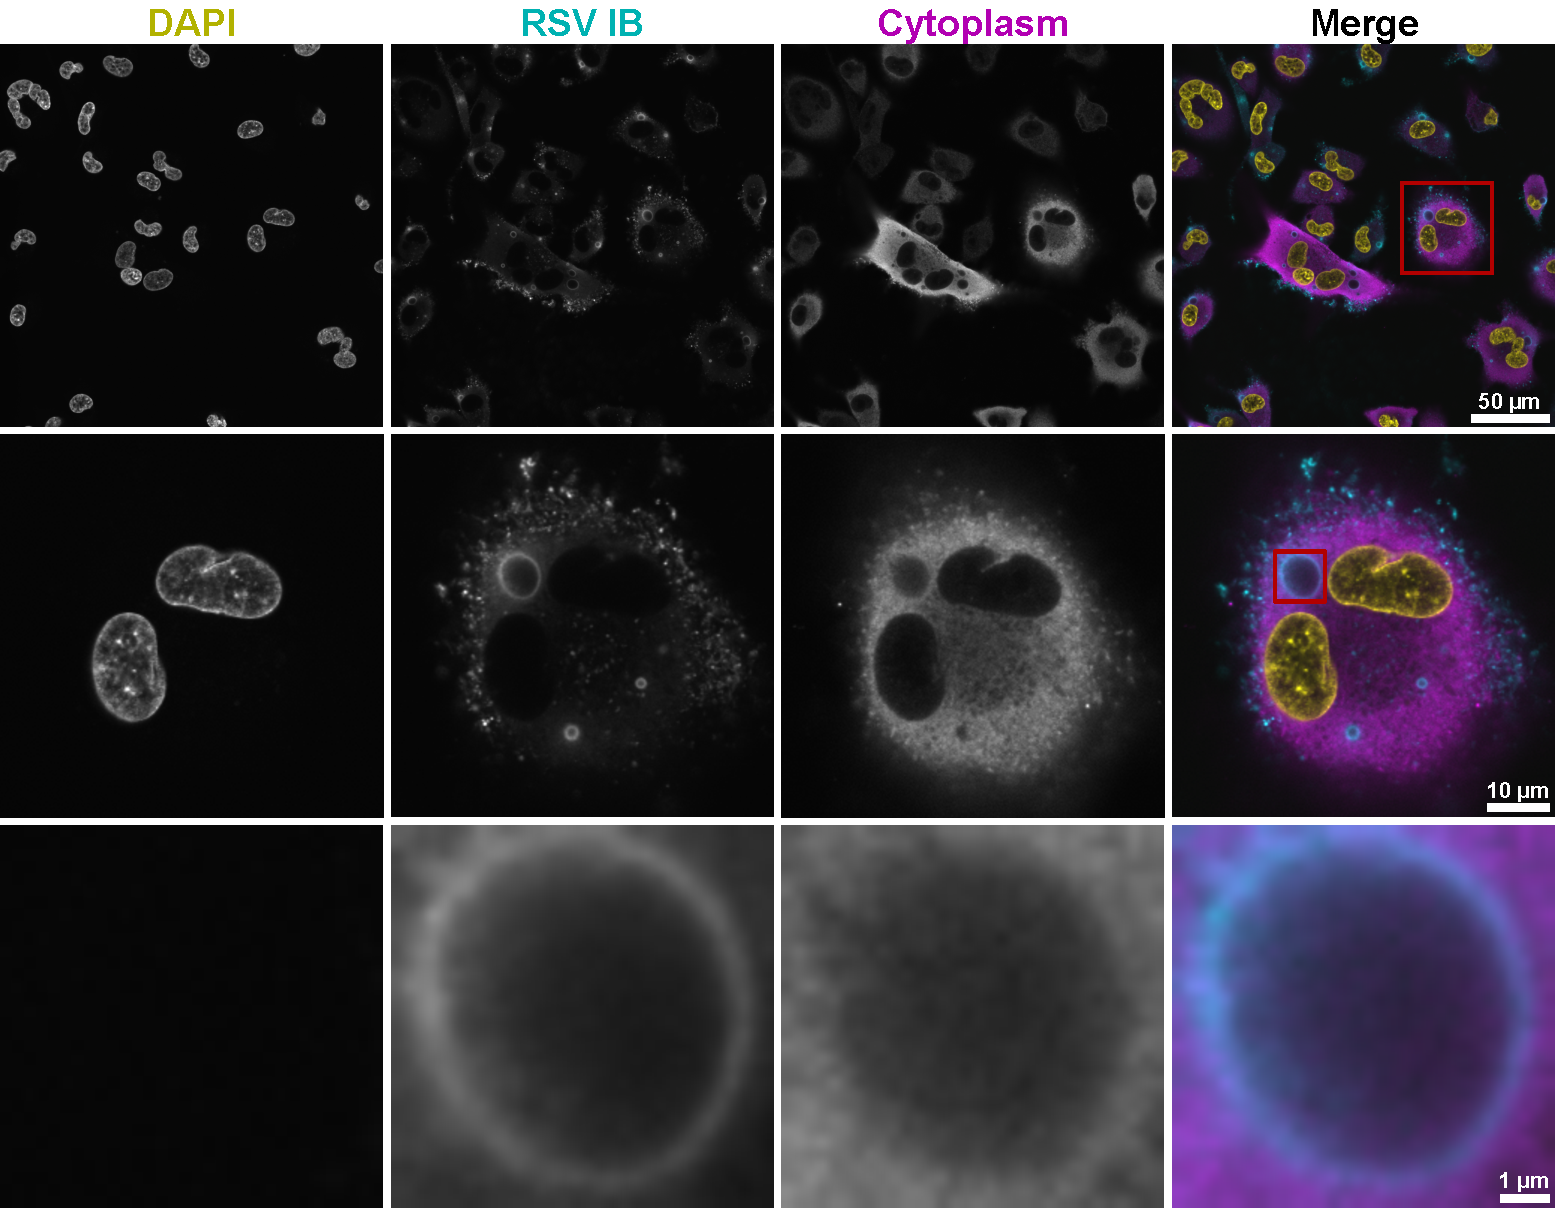
\includegraphics[width=1\linewidth]{08. Chapter 3/Figs/01. Localisation introduction/01. IB-zooms.pdf}
    \caption[Inclusion Bodies Within RSV Infected Cells: Zoom Sequence.]{\textbf{Inclusion Bodies Within RSV Infected Cells: Zoom Sequence.} A represerenative image of RSV infected cells detected using confocal microscopy. Cellular nuclei were stained with DAPI and are shown in yellow; RSV inclusion bodies are shown in cyan; and the cytoplasm is shown in magenta. Figure highlights a zoom sequence from a population of cells, into a single syncytia view, with lastly focusing at one individual inclusion body.}
    \label{fig:Inclusion Bodies Within RSV Infected Cells: Zoom Sequence}
\end{figure}

 We observed and annotated 1727 inclusion bodies between the different cell lines in terms of their IFIT interaction phenotypes as described above, and their radia (\(\mu \mbox{m}\)) and area (\(\mu \mbox{m}^2\)) as deteted by the observed 2D projections. In more detail, we observed 1008 hRSV IBs in A549 cell line; 99 hRSV IBs in BEAS2B cell line; and 620 bRSV IBs in MDBK cell line. Figure \ref{fig:Size Characterization of Inclusion Bodies Across Different Cell Lines} highlights the relationship between the IB area and radius either as an aggregate of all observed IBs, or of IBs detected per cell line. We can see both the aggregate and the individual cell line data broadly follows a logarithmic curve, as one can expect, suggesting that the majority of the IBs are circular in shape. We also see a deviation from this pattern in each cell line, especially in lasrger IBs, where the area increases inproportionatly with the radius, suggesting a more elongated elipsiod shape of these IBs. We can also see that most IBs, regardless of the origin, seem to confort to the area of bellow 10 \(\mu \mbox{m}^2\). In terms of the most common radia, both BEAS2B and MDBK IBs have the tendency to be bellow 1 \(\mu \mbox{m}\), while the A549 IBs display a range of the most common radia size of between 0.5 and 1.5 \(\mu \mbox{m}\). A more detailed view of the distribution of the measured areas per cell line can be seen in Figure \ref{fig:The Distributions of IB Areas Observed Per Cell Line}. There we can see that all 3 cell lines accompass IBs ranging from sub 0.5 \(\mu \mbox{m}^2\) to supra 30 \(\mu \mbox{m}^2\), with the median sizes of 5 \(\mu \mbox{m}^2\), 3 \(\mu \mbox{m}^2\), and 2 \(\mu \mbox{m}^2\) for A549, BEAS2B, and MDBK respectivelly. We observed the most sub 1 \(\mu \mbox{m}^2\) IBs in the MDBK cell line, while A549 had the most supra 10 \(\mu \mbox{m}^2\) IBs.

\begin{figure}
    \begin{subfigure}{0.495\textwidth}
        \caption{}
        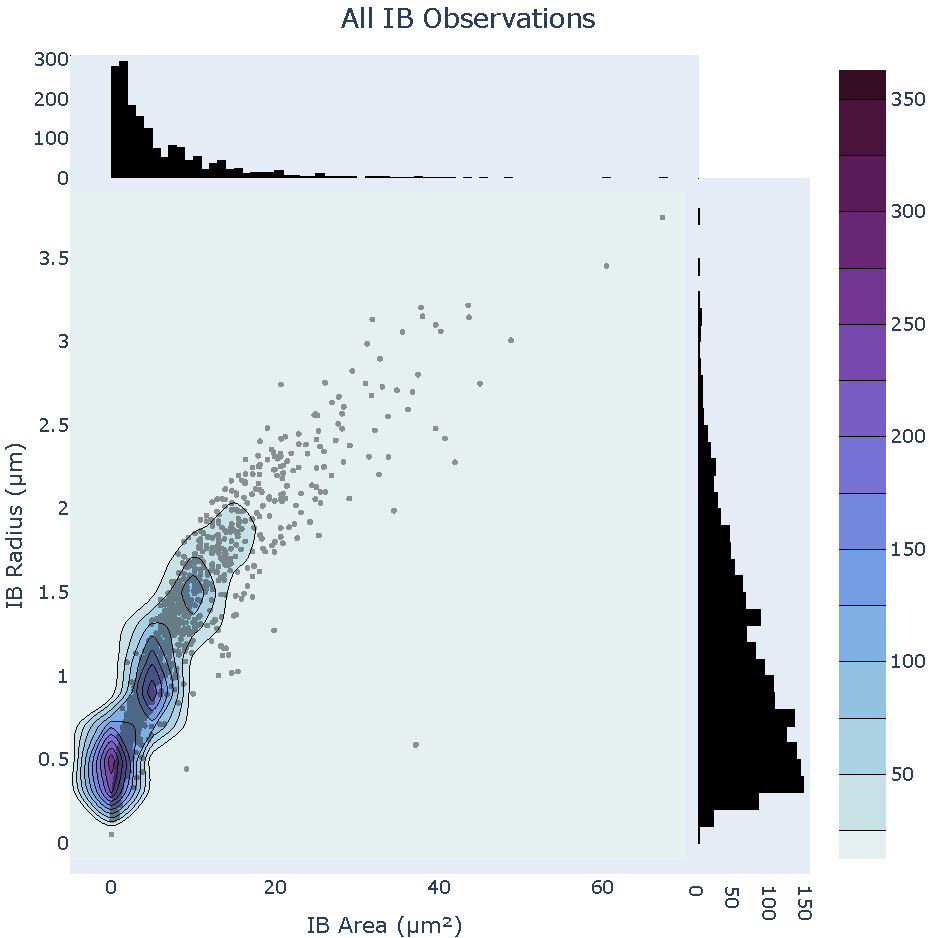
\includegraphics[width=\textwidth]{08. Chapter 3/Figs/01. Localisation introduction/02. heatmap_all.pdf} 
    \end{subfigure}
    \hfill
    \begin{subfigure}{0.495\textwidth}
        \caption{}
        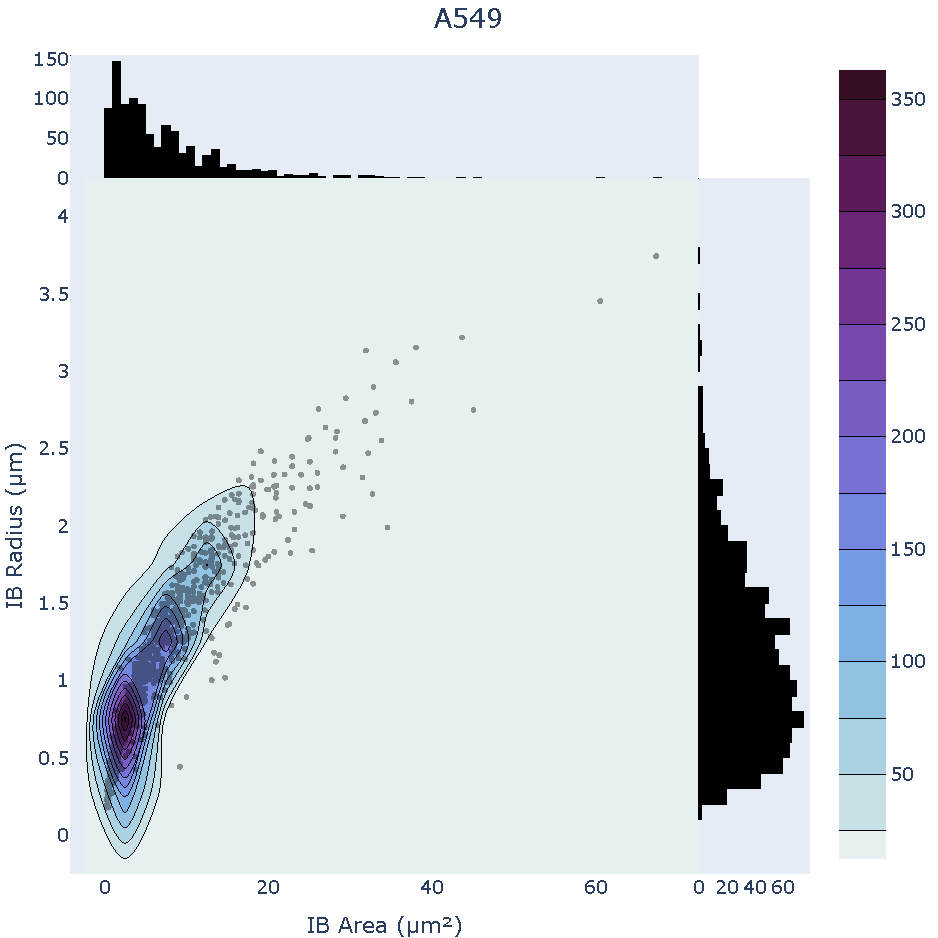
\includegraphics[width=\textwidth]{08. Chapter 3/Figs/01. Localisation introduction/03. heatmap_a549.pdf}
    \end{subfigure}

    \medskip
    \begin{subfigure}{0.495\textwidth}
        \caption{}
        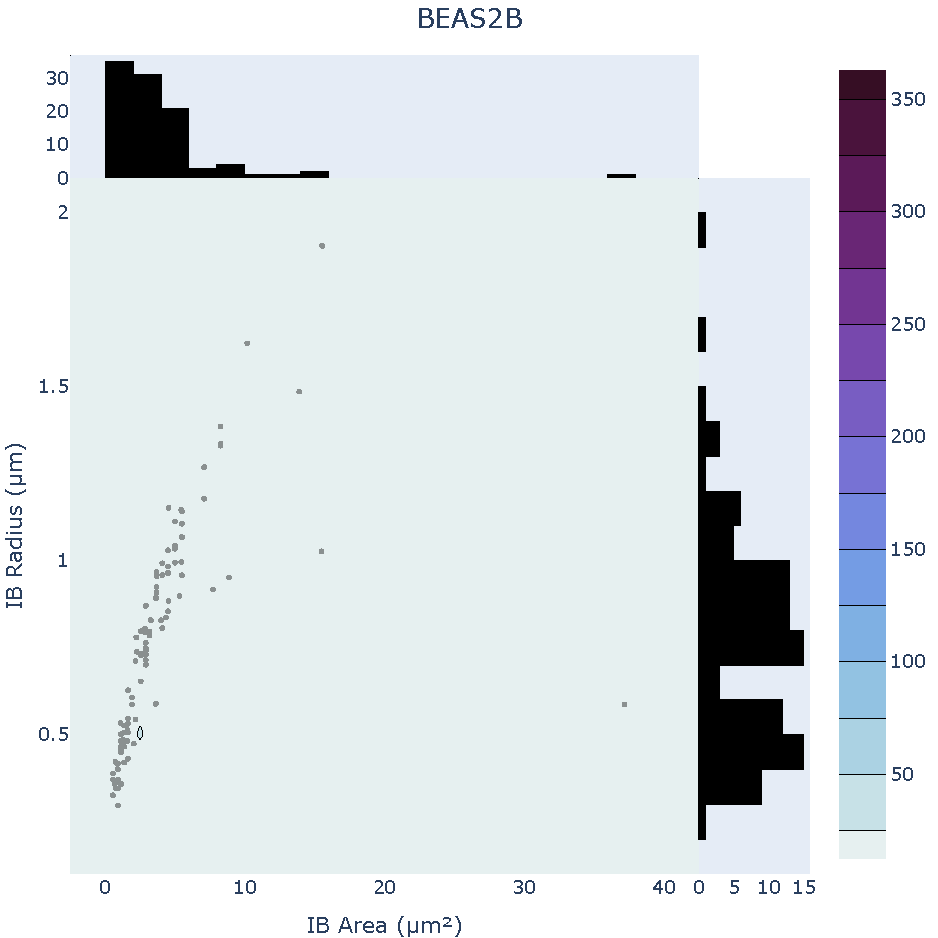
\includegraphics[width=\textwidth]{08. Chapter 3/Figs/01. Localisation introduction/04. heatmap_beas2b.pdf} 
    \end{subfigure}
    \hfill
    \begin{subfigure}{0.495\textwidth}
        \caption{}
        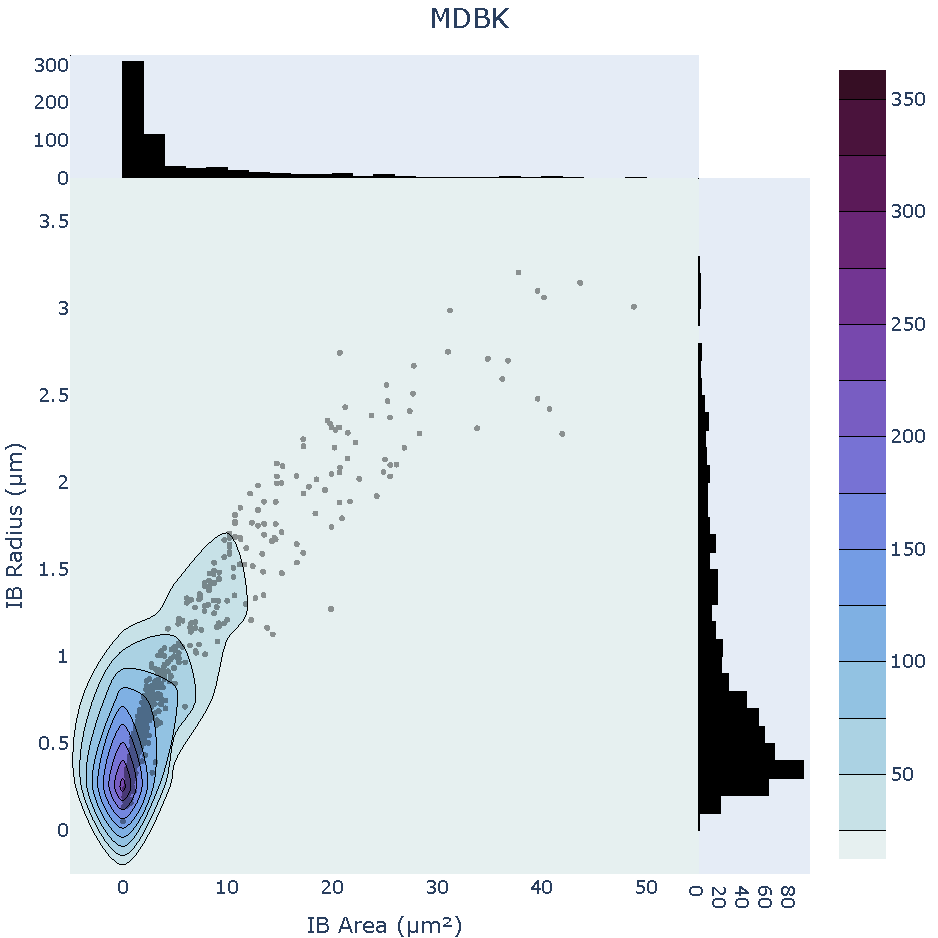
\includegraphics[width=\textwidth]{08. Chapter 3/Figs/01. Localisation introduction/05. heatmap_mdbk.pdf} 
    \end{subfigure}
    
    \caption[Size Characterization of Inclusion Bodies Across Different Cell Lines.]{\textbf{Size Characterization of Inclusion Bodies Across Different Cell Lines.} This figure presents the relationship between the measured area (\(\mu \mbox{m}^2\)) and radius (\(\mu \mbox{m}\)) of individual inclusion bodies (IBs) as observed within the scope of this study. Additionally, the figure includes distinct population distributions depicted alongside the plots, representing (a) the aggregate of 1727 observations of IBs across all individual cell lines, (b) 1008 observations from the A549 cell line, (c) 99 observations from the BEAS2B cell line, and (d) 620 observations from the MDBK cell line. Contour plots are incorporated to elucidate the underlying density of individual IBs within the plots.}
    \label{fig:Size Characterization of Inclusion Bodies Across Different Cell Lines}  
\end{figure}

From the published literature we know that increasing IB area is correlative with its matruation state and internal complexity. We know that IBs that contain IBAGs are significantly larger than those without (6.4 \(\mu \mbox{m}^2\) versus 2.3 \(\mu \mbox{m}^2\)) in HEp-2 cell line infected with hRSV \cite{Rincheval2017FunctionalVirus}. We also know that in MDBk cell line, during early infection timepoint (6h) only small IBs are present (mean value of 1 \(\mu \mbox{m}^2\)), which do not contain IBAGs. At 16 HPI the IBAG-less retain the mean area value, while larger IBs with IBAGs (mean area of 10 \(\mu \mbox{m}^2\)) are also present \cite{Jobe2021BovineResponses}. At 24 HPI, a timepoint important for the analysis in this thesis, small IBAG-less IBs retain the median size of 1 \(\mu \mbox{m}^2\), while the larger, IBAG-containg IBs cluster in two sizes, with the mean areas of 2.5 \(\mu \mbox{m}^2\) and 17 \(\mu \mbox{m}^2\). Based on this information we can assess the observed IFIT-IB interaction phenotypes per mature or immature IBs.

\begin{figure}
    \centering
    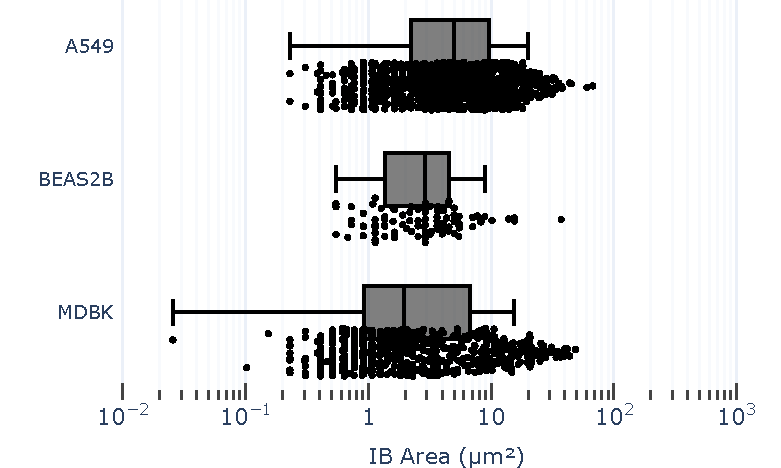
\includegraphics[width=1\linewidth]{08. Chapter 3/Figs/01. Localisation introduction/06. box-infection.pdf}
    \caption[The Distributions of IB Areas Observed Per Cell Line.]{\textbf{The Distributions of IB Areas Observed Per Cell Line.} The distribution of RSV inclusion body areas (\(\mu \mbox{m}^2\)), detected in this study are shown. 1008 observations were made in A549 cell line, 99 observations were made in BEAS2B cell line, and 620 observations were from MDBK cell line.}
    \label{fig:The Distributions of IB Areas Observed Per Cell Line}
\end{figure}